%% LyX 2.3.4.2 created this file.  For more info, see http://www.lyx.org/.
%% Do not edit unless you really know what you are doing.
\documentclass[english,dvipsnames,aspectratio=169]{beamer}
\usepackage{mathptmx}
\usepackage{eulervm}
\usepackage[T1]{fontenc}
\usepackage[latin9]{inputenc}
\usepackage{babel}
\usepackage{amstext}
\usepackage{amssymb}
\usepackage{graphicx}
\usepackage{ifthen}
\usepackage{xcolor}
\usepackage{xspace}
\usepackage{tikz}
\usetikzlibrary{tikzmark}
\usetikzlibrary{calc}
\usepackage{pgfplots}
%\pgfplotsset{compat=1.17}
\usepackage{booktabs}
\usepackage{xpatch}

\xpatchcmd{\itemize}
  {\def\makelabel}
  {\ifnum\@itemdepth=1\relax
     \setlength\itemsep{2ex}% separation for first level
   \else
     \ifnum\@itemdepth=2\relax
       \setlength\itemsep{1ex}% separation for second level
     \else
       \ifnum\@itemdepth=3\relax
         \setlength\itemsep{0.5ex}% separation for third level
   \fi\fi\fi\def\makelabel
  }
 {}
 {}

\ifx\hypersetup\undefined
  \AtBeginDocument{%
    \hypersetup{unicode=true,pdfusetitle,
 bookmarks=true,bookmarksnumbered=false,bookmarksopen=false,
 breaklinks=false,pdfborder={0 0 0},pdfborderstyle={},backref=false,colorlinks=true,
 allcolors=NYUPurple,urlcolor=LightPurple}
  }
\else
  \hypersetup{unicode=true,pdfusetitle,
 bookmarks=true,bookmarksnumbered=false,bookmarksopen=false,
 breaklinks=false,pdfborder={0 0 0},pdfborderstyle={},backref=false,colorlinks=true,
 allcolors=NYUPurple,urlcolor=LightPurple}
\fi

\makeatletter

%%%%%%%%%%%%%%%%%%%%%%%%%%%%%% LyX specific LaTeX commands.
%% Because html converters don't know tabularnewline
\providecommand{\tabularnewline}{\\}

%%%%%%%%%%%%%%%%%%%%%%%%%%%%%% Textclass specific LaTeX commands.
% this default might be overridden by plain title style
\newcommand\makebeamertitle{\frame{\maketitle}}%
% (ERT) argument for the TOC
\AtBeginDocument{%
  \let\origtableofcontents=\tableofcontents
  \def\tableofcontents{\@ifnextchar[{\origtableofcontents}{\gobbletableofcontents}}
  \def\gobbletableofcontents#1{\origtableofcontents}
}

%%%%%%%%%%%%%%%%%%%%%%%%%%%%%% User specified LaTeX commands.
\usetheme{CambridgeUS} 
\beamertemplatenavigationsymbolsempty


% Set Color ==============================
\definecolor{NYUPurple}{RGB}{87,6,140}
\definecolor{LightPurple}{RGB}{165,11,255}


\setbeamercolor{title}{fg=NYUPurple}
\setbeamercolor{frametitle}{fg=NYUPurple}

\setbeamercolor{background canvas}{fg=NYUPurple, bg=white}
\setbeamercolor{background}{fg=black, bg=NYUPurple}

\setbeamercolor{palette primary}{fg=black, bg=gray!30!white}
\setbeamercolor{palette secondary}{fg=black, bg=gray!20!white}
\setbeamercolor{palette tertiary}{fg=gray!20!white, bg=NYUPurple}

\setbeamertemplate{headline}{}
\setbeamerfont{itemize/enumerate body}{}
\setbeamerfont{itemize/enumerate subbody}{size=\normalsize}

\setbeamercolor{parttitle}{fg=NYUPurple}
\setbeamercolor{sectiontitle}{fg=NYUPurple}
\setbeamercolor{sectionname}{fg=NYUPurple}
\setbeamercolor{section page}{fg=NYUPurple}
%\setbeamercolor{description item}{fg=NYUPurple}
%\setbeamercolor{block title}{fg=NYUPurple}

\setbeamertemplate{blocks}[rounded][shadow=false]
\setbeamercolor{block body}{bg=normal text.bg!90!NYUPurple}
\setbeamercolor{block title}{bg=NYUPurple!30, fg=NYUPurple}



\AtBeginSection[]{
  \begin{frame}
  \vfill
  \centering
\setbeamercolor{section title}{fg=NYUPurple}
 \begin{beamercolorbox}[sep=8pt,center,shadow=true,rounded=true]{title}
    \usebeamerfont{title}\usebeamercolor[fg]{title}\insertsectionhead\par%
  \end{beamercolorbox}
  \vfill
  \end{frame}
}

\makeatother

\setlength{\parskip}{\medskipamount} 

\input ../macros

\begin{document}
\input ../rosenberg-macros

\title[DS-GA 1003]{Gradient Descent}
\author{He He}
\date{Feb 9, 2021}
\institute{CDS, NYU}

\makebeamertitle
\mode<article>{Just in article version}

\section{Review: ERM}
\begin{frame}{Our Setup from Statistical Learning Theory}
\begin{block}{The Spaces}
\begin{columns}[t]

\column{.3\textwidth}
\begin{itemize}
\item $\cx$: input space
\end{itemize}

\column{.3\textwidth}
\begin{itemize}
\item $\cy$: outcome space 
\end{itemize}

\column{.3\textwidth}
\begin{itemize}
\item $\ca$: action space
\end{itemize}
\end{columns}

\end{block}

\begin{block}{Prediction Function (or ``decision function'')}

A \textbf{prediction function }(or \textbf{decision function}) gets
input $x\in\cx$ and produces an action $a\in\ca$ :

\[
\begin{matrix}f: & \cx & \rightarrow & \ca\\
 & x & \mapsto & f(x)
\end{matrix}
\]
\end{block}
\begin{block}{Loss Function}

A \textbf{loss function} evaluates an action in the context of the
outcome $y$.

\[
\begin{matrix}\loss: & \ca\times\cy & \rightarrow & \reals\\
& (a,y) & \mapsto & \loss(a,y)
\end{matrix}
\]

\end{block}
\end{frame}
%
\begin{frame}{Risk and the Bayes Prediction Function }
\begin{definition}
The \textbf{risk}\emph{ }of a prediction function $f:\cx\to\ca$ is
\[
R(f)=\ex\loss(f(x),y).
\]
In words, it's the \textbf{expected loss} of $f$ on a new exampe
$(x,y)$ drawn randomly from $P_{\cx\times\cy}$.
\end{definition}


\begin{definition}
A \textbf{Bayes prediction function} $\minimizer f:\cx\to\ca$ is
a function that achieves the \emph{minimal risk} among all possible
functions: 
\[
\minimizer f\in\argmin_{f}R(f),
\]
where the minimum is taken over all functions from $\cx$ to $\ca$. 
\end{definition}

\begin{itemize}
\item The risk of a Bayes prediction function is called the \textbf{Bayes
risk}.
\end{itemize}
\end{frame}
%
\begin{frame}{The Empirical Risk}

Let $\cd_{n}=\left((x_{1},y_{1}),\ldots,(x_{n},y_{n})\right)$ be
drawn i.i.d. from $\cp_{\cx\times\cy}$.
\begin{definition}
The \textbf{empirical risk}\emph{ }of $f:\cx\to\ca$ with respect
to $\cd_{n}$ is
\[
\hat{R}_{n}(f)=\frac{1}{n}\sum_{i=1}^{n}\loss(f(x_{i}),y_{i}).
\]
\end{definition}


\begin{itemize}
\item But we saw that the \textbf{unconstrained} empirical risk minimizer
overfits.

\begin{itemize}
\item i.e. if we minize $\hat{R}_{n}(f)$ over\textbf{ all functions}, we
overfit. 
\end{itemize}
\end{itemize}
\end{frame}
%
\begin{frame}{Constrained Empirical Risk Minimization}
\begin{definition}
A \textbf{hypothesis space} $\cf$ is a set of functions mapping $\cx\to\ca$.
\begin{itemize}
\item It is the collection of prediction functions we are choosing from.
\end{itemize}
\end{definition}

\begin{itemize}
\item \textbf{Empirical risk minimizer }(ERM) in $\cf$ is 
\[
\hat{f}_{n}\in\argmin_{f\in\cf}\frac{1}{n}\sum_{i=1}^{n}\loss(f(x_{i}),y_{i}).
\]

\item From now on ``ERM'' always means ``constrained ERM''.
\item So we should always specify the hypothesis space when we're doing
ERM.
\end{itemize}
\end{frame}
%
\begin{frame}{Example: Linear Least Squares Regression}
\begin{block}{Setup}
\begin{itemize}
\item Input space $\cx=\reals^{d}$
\item Output space $\cy=\reals$
\item Action space $\cy=\reals$
\end{itemize}

\begin{itemize}
\item Loss: $\loss(\hat{y},y)=\left(y-\hat{y}\right)^{2}$
\item \textbf{Hypothesis space:} $\cf=\left\{ f:\reals^{d}\to\reals\mid f(x)=w^{T}x\,,\,w\in\reals^{d}\right\} $
\end{itemize}

\end{block}
\begin{itemize}
\item Given data set $\cd_{n}=\left\{ (x_{1},y_{1}),\ldots,(x_{n},y_{n})\right\} $,
\begin{itemize}
\item Let's find the ERM $\hat{f}\in\cf$. 
\end{itemize}
\end{itemize}
\end{frame}

\begin{frame}{Example: Linear Least Squares Regression}
\begin{block}{Objective Function: Empirical Risk}

The function we want to minimize is the empirical risk:
\[
\hat{R}_{n}(w)=\frac{1}{n}\sum_{i=1}^{n}\left(w^{T}x_{i}-y_{i}\right)^{2},
\]
where $w\in\reals^{d}$ parameterizes the hypothesis space $\cf$.

\end{block}
\begin{itemize}
\item Now, we have ended up with an optimization problem:
    $$
        \min_{w\in\reals^d} \hat{R}_n(w) .
        $$
\end{itemize}
\end{frame}

\section{Gradient Descent}

\begin{frame}{Unconstrained Optimization}
\begin{block}{Setting}

Objective function $f:\reals^{d}\to\reals$ is \emph{differentiable.}

Want to find 
\[
x^{*}=\arg\min_{x\in\reals^{d}}f(x)
\]
\end{block}
\end{frame}

\begin{frame}{The Gradient}
\begin{itemize}
\item Let $f:\reals^{d}\to\reals$ be differentiable at $x_{0}\in\reals^{d}$.
\end{itemize}

\begin{itemize}
\item The \textbf{gradient} of $f$  at the point $x_{0}$, denoted $\del_{x}f(x_{0})$,
is the direction to move in for the \textbf{fastest increase} in $f(x)$,
when starting from $x_{0}$.
\end{itemize}
\begin{center}
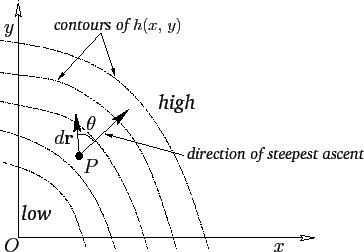
\includegraphics[height=0.4\textheight]{figures/two-dim-gradient}
\par\end{center}

\let\thefootnote\relax\footnotetext{\tiny{Figure A.111 from Newtonian Dynamics, by Richard Fitzpatrick.}}
\end{frame}

\begin{frame}{Gradient Descent}
\begin{block}{Gradient Descent}
\begin{itemize}
\item Initialize $x=0$
\item repeat 
\begin{itemize}
\item $x\gets x-\underbrace{\eta}_{\mbox{step size}}\del f(x)$
\end{itemize}
\item until stopping criterion satisfied
\end{itemize}
\end{block}
Choosing the step size is the key in gradient descent.
\end{frame}

\begin{frame}{Gradient Descent Path}
\begin{center}
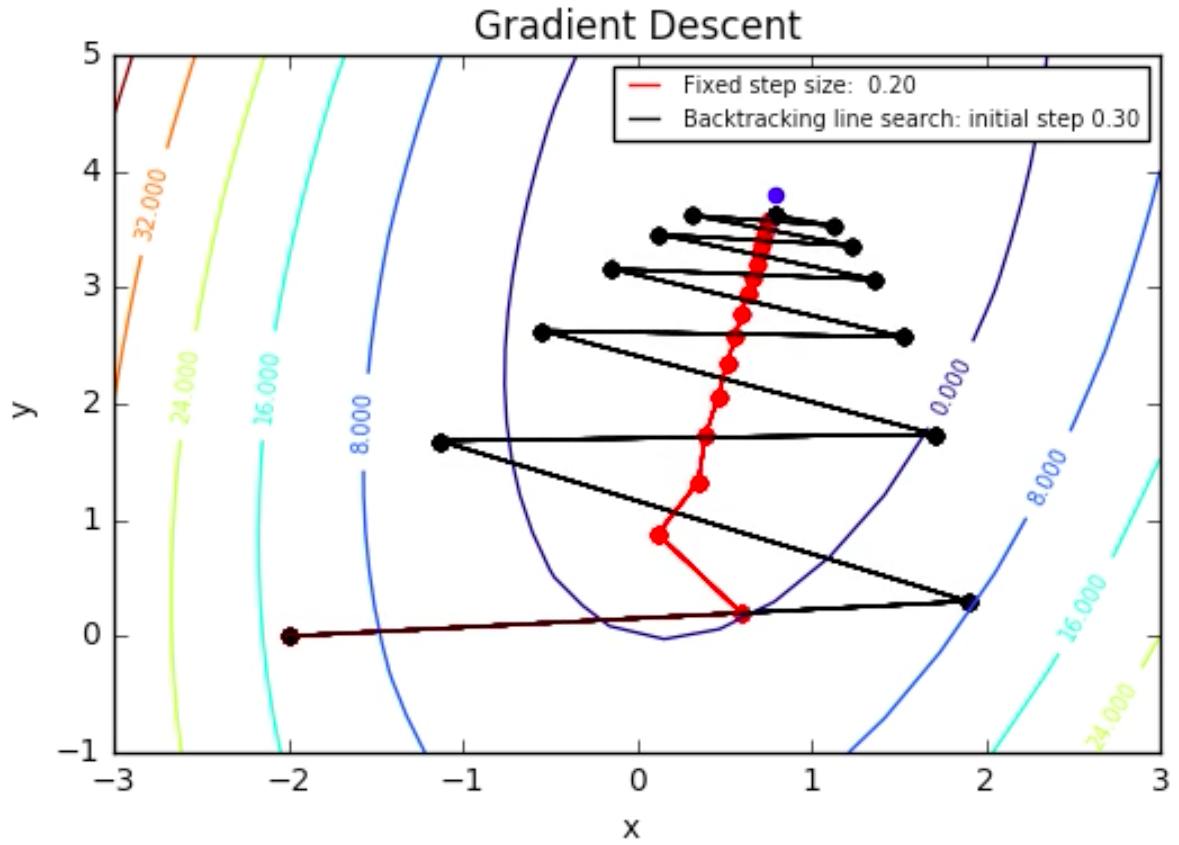
\includegraphics[height=0.8\textheight]{figures/vlad-GD-fixedAndBacktracking} 
\par\end{center}

\end{frame}

\begin{frame}{Gradient Descent: Step Size}
\begin{itemize}
\item A fixed step size will work, eventually, as long as it's small enough
(roughly - details to come)
\begin{itemize}
\item Too fast, may diverge
\item In practice, try several fixed step sizes
\end{itemize}
\end{itemize}

\begin{itemize}
\item Intuition on when to take big steps and when to take small steps?
    \vspace{4em}
\end{itemize}
\end{frame}
%
\begin{frame}{Convergence Theorem for Fixed Step Size}
\begin{theorem}
Suppose $f:\reals^{d}\to\reals$ is convex and differentiable, and
$\del f$ is \textbf{Lipschitz continuous} with constant $L>0$, i.e.
\[
\|\del f(x)-\del f(x')\|\le L\|x-x'\|
\]
for any $x,x'\in\reals^{d}$. Then gradient descent with
fixed step size $\eta\le1/L$ \textbf{converges}. In particular,
\[
f(x^{(k)})-f(x^{*})\le\frac{\|x^{(0)}-x^{*}\|^{2}}{2\eta k}.
\]
\mode<article>{Proof sketch: Fit a quadratic at $x$ that's tangent to $f(x)$ and
has Lipschitz constant $L$. Taylor remainder theorem to show that
$f(x)$ is below quadratic. Jump to minimizer of quadratic.} 

\end{theorem}

This says that gradient descent is guaranteed to converge and that it converges with rate $O(1/k)$.
\end{frame}
%

\begin{frame}{Gradient Descent: When to Stop?}
\begin{itemize}
\item Wait until $\|\del f(x)\|_{2}\leq\eps$, for some $\eps$ of your
choosing.
\begin{itemize}
\item (Recall $\del f(x)=0$ at minimum.)
\end{itemize}
\end{itemize}

\begin{itemize}
\item For learning setting,
\begin{itemize}
\item evalute performance on validation data as you go
\item stop when not improving, or getting worse
\end{itemize}
\end{itemize}
\end{frame}


\end{document}
